\phantomsection
\addcontentsline{toc}{chapter}{Appendices}

% The \appendix command resets the chapter counter, and changes the chapter numbering scheme to capital letters.
%\chapter{Appendices}
\appendix

\chapter{pyKrack}
\label{appendix:pykrack}

\section{Introduction}

Biological signalling can be modelled as a directed network, where nodes represent genes/proteins and edges represent signalling interactions.

The hierarchy of such a network can be quantified using various metrics, including the Krackhardt hierarchy score. This score measures the degree to which the network exhibits a perfect hierarchy, with higher scores indicating greater hierarchy.

In R the sna package presents methods to compute graph hierarchy including Krackhardt’s score, and there are other hierarchy scores implemented in Python such as Flow Hierarchy Score~\cite{luo_detecting_2011}. However, despite its utility, there is currently no native implementation of the Krackhardt hierarchy score in Python.

\subsection{Krackhardt Hierarchy Score}

The Krackhard hierarchy score was introduced by David Krackhardt [Krackhardt, David. (1994). Graph Theoretical Dimensions of Informal Organization. Computational Organization Theory. 89], where he defined it in the following way:

\begin{quote}
    \emph{The graph hierarchy condition states that in a digraph D, for each pair of points where one (Pi) can reach another (Pj), the second (Pj) can't reach the first (Pi). 
    For example, in a formal organization chart a high level employee can reach through the chain of command her subordinate's subordinate. If the formal organization is working "properly", this lower level employee can't simultaneously reach the high level employee.
    To measure the degree of hierarchy of digraph D, a new digraph Dr must be created. Dr is defined as the reachability digraph of D. Each point in D exists in Dr; moreover, the line (Pi,Pj) exists in Dr if and only if Pi can reach Pj in D. If D is graph hierarchic, then Dr will have no symmetric lines in it (i.e. if the line (Pi,Pj) exists in Dr then the line (Pj,Pi) does not)}.
\end{quote}

The degree of hierarchy then is defined as \[Graph Hierarchy = 1 - [V/MaxV]\]
where $V$ is the number of unordered pairs of points in Dr that are symmetrically linked and $MaxV$ the number of unordered pairs of points in $Dr$ where $Pi$ is linked to $Pj$ or viceversa.

\section{Hierarchy Computation}

Based on the definition above, I wrote a small Python package to compute the Krackhardt hierarchy score. Built around a main function that computes the hierarchy score (Listing \ref{lst:pykrack}), the pykrack package (\url{ferranc96.github.io/pyKrack}) also includes a helper function to describe general properties of a directed graph and computes an alternative hierarchy score.

\label{lst:pykrack}
\begin{lstlisting}[language=Python, caption=\textbf{Main pyKrack function}. The \emph{compute\_hierarchy} function takes in a directed graph and computes its hierarchy flow score or the Krackhardt hierarchy score using an existing R implementation or a novel one in Python.]

def compute_hierarchy(G, metric="pykrack"):
    """
    Compute one of the possible hierarchy scores
    
    Parameters
    ----------
    G
        Directed NetworkX graph
    metric : str
        Type of hierarchy metric to compute. Accepted types are:
        'pykrack' for this module's implementation of the Krackhardt score.
        'rsnakrack' for the sna implementation in R.
        'hierarchy_flow' for the Luo and Magee 2011 as implemented in the NetworkX package.

    Returns
    -------
    score : float
        One of the possible hierarchy scores
    """

    #Ensure Graph is DirectedGraph
    if not G.is_directed():
        raise Exception
    #Ensure Graph is of DiGraph() format
    G = nx.DiGraph(G)

    if metric == "pykrack": #Python implementation
        #Compute transitive closure of graph to get the reachability graph
            #[contains an edge (i,j) if there is a path from i to j in the original graph]
        acyclic = 0
        try:
            nx.find_cycle(G)
        except:
            print("Acyclic graph")
            acyclic = 1
        if acyclic == 1:
            Gr = nx.transitive_closure_dag(G)
        else:
            Gr = nx.transitive_closure(G, reflexive=None)
        symmetric_dyads = 0
        non_null_dyads = 0
        n = len(Gr.nodes())
        #Count the number of non-null symmetric dyads
        for pair in product(Gr.nodes(), Gr.nodes()):
            if Gr.has_edge(pair[0],pair[1]) or Gr.has_edge(pair[1],pair[0]): #Non-null dyad
                non_null_dyads+=1
                if  Gr.has_edge(pair[0],pair[1]) == Gr.has_edge(pair[1],pair[0]): #Symmetric!
                    symmetric_dyads+=1
        #Raise exception if graph has no edges!
        if non_null_dyads == 0:
            raise Exception
        score = 1 - (symmetric_dyads / non_null_dyads)
    
    elif metric == "rsnakrack": #R implementation from the sna package
        try:
            base = importr("base")
            sna = importr("sna")
            score = sna.hierarchy(nx.to_numpy_array(G), measure="krackhardt")[0]
        except:
            print("R package sna was not found. Please install manually!")
            print("Computing hierarchy flow instead")
            snafail_flag = 1
            score = nx.flow_hierarchy(G)
    
    elif metric == "hierarchy_flow": #Networkx's hierarchy flow implementation
        score = nx.flow_hierarchy(G)

    # elif metric == "all": #This will eventually return a dict with all metrics

    else: # metric argument broken
        raise Exception


    return score

\end{lstlisting}

\section{Notebook-Centric Implementation}

This package has been implemented using the nbdev framework (\url{nbdev.fast.ai}). This technology allows for a notebook-centric approach to software development and distribution, including automation of documentation sites to continuous integration actions that automate package releases.

I have leveraged nbdev to publish this tool as a package in Pypi (\url{pypi.org/project/pykrack}), and as a technology demonstrator for an upcoming deployment of the \acrshort{vr} score landscapes.



\chapter{Supplementary Figures}
\label{appendix:SupFig}

\section{Figures related to Chapter \ref{04seq}}

\begin{figure}[h!]
    \centering
    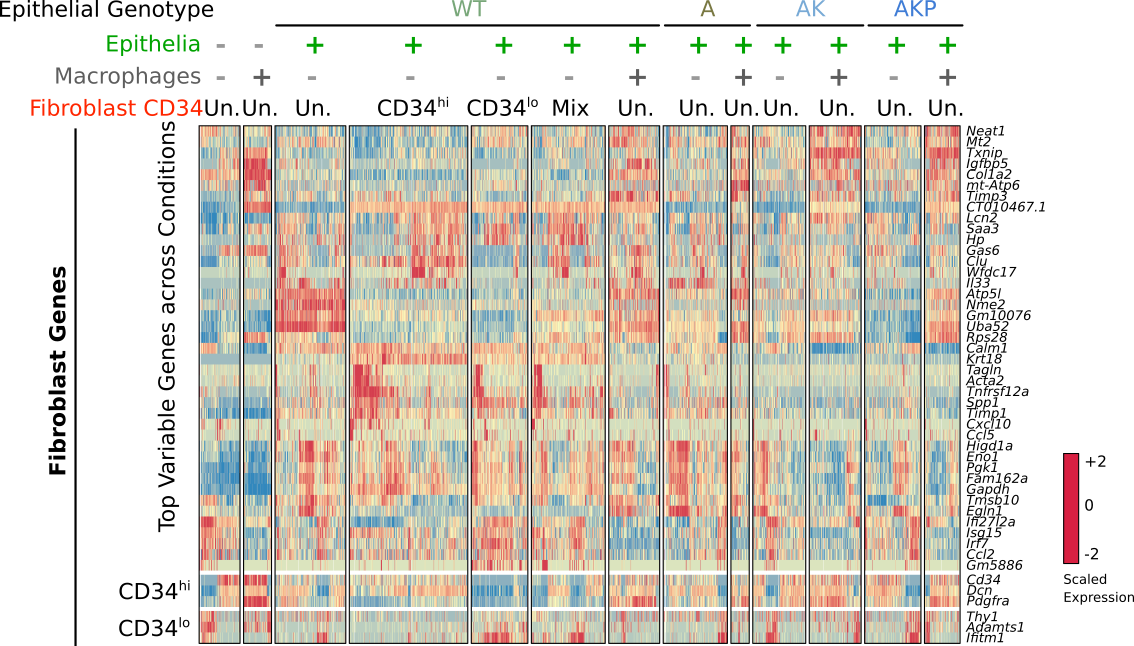
\includegraphics{0Xappendices/0XSup_DEfib.png}
    \caption{\textbf{Fibroblast DE Analysis.} Differential gene expression analysis of fibroblasts regulated by epithelial organoids and macrophages.}
    \label{fig:defib}
\end{figure}

\begin{figure}[h!]
    \centering
    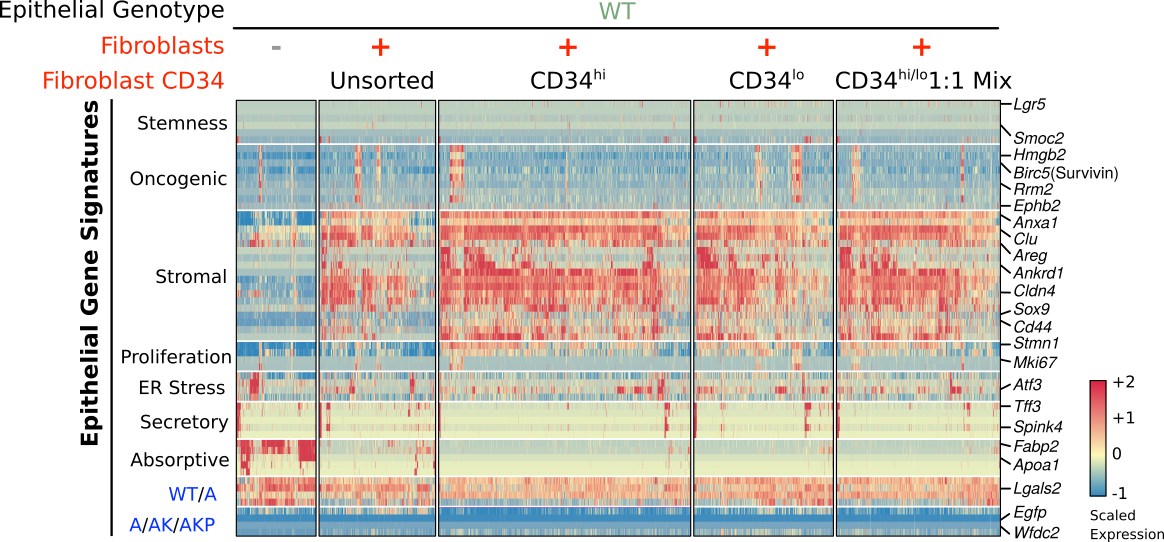
\includegraphics{0Xappendices/0XSup_DEepibyfib.png}
    \caption{\textbf{Epithelial DE Analysis by Fibroblast-Subtype.} Differential gene expression analysis of \acrshort{wt} colonic organoids co-cultured with unsorted, CD34\textsuperscript{hi}, CD34\textsuperscript{lo}, and a 1:1 mix of CD34\textsuperscript{hi}:CD34\textsuperscript{hi} colonic fibroblasts.}
    \label{fig:deepibyfib}
\end{figure}

\begin{figure}[h!]
    \centering
    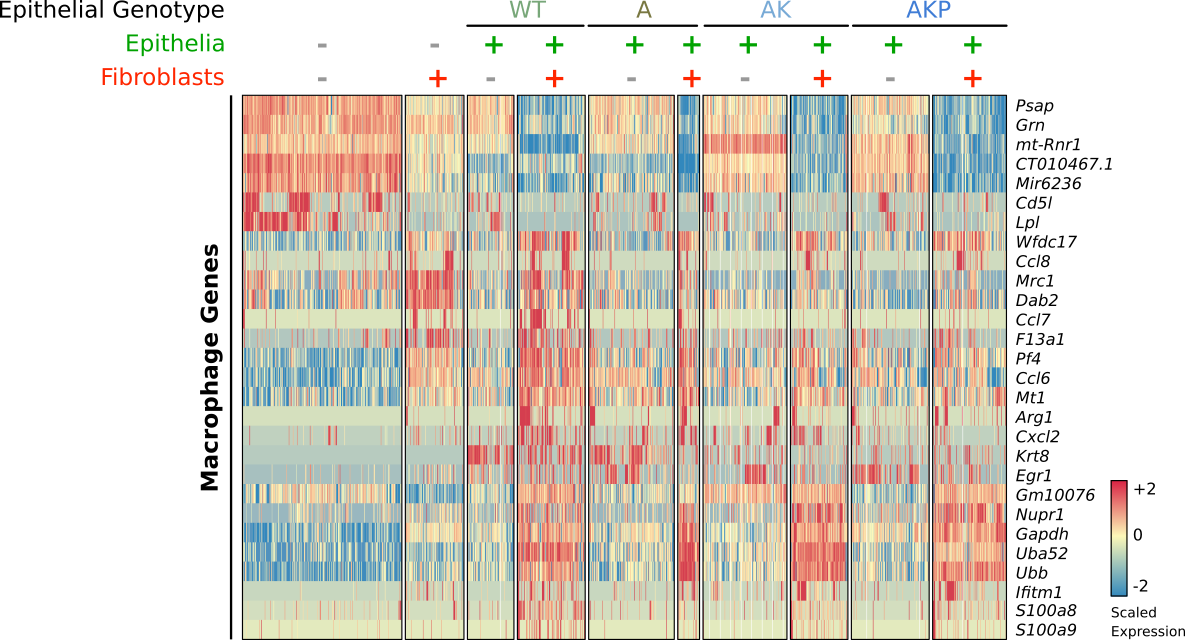
\includegraphics{0Xappendices/0XSup_DEmac.png}
    \caption{\textbf{Macrophages DE Analysis.} Differential gene expression analysis of macrophages regulated by epithelial organoids and fibroblasts}
    \label{fig:demac}
\end{figure}

\chapter{Supplementary Tables}
\label{appendix:SupTab}

\section{Gene Data}

\newpage
\begin{table}[H]
  \centering
  \caption{\textbf{Colonic Epithelia Gene Markers (1/2)}. Markers of epithelial populations and organoid genotypes. Derived from literature and DE analysis of our data.}
  \label{tab:epimarkers}
  \csvreader[
    tabular=|c|c|,
    head=true,
    table head=\hline \textbf{Gene} & \textbf{Annotation}\\ \hline,
    late after line=\\ \hline,
    filter={\value{csvinputline}<30},
    separator=comma,
    respect all
  ]{0Xappendices/CuratedEpithelia_geneSet.csv}{}
  {\csvcoli & \csvcolii}
\end{table}
\newpage
\begin{table}[H]
  \centering
  \caption{\textbf{Colonic Epithelia Gene Markers (2/2)}.}
  \csvreader[
    tabular=|c|c|,
    head=true,
    table head=\hline \textbf{Gene} & \textbf{Annotation}\\ \hline,
    late after line=\\ \hline,
    filter={\value{csvinputline}>29},
    separator=comma,
    respect all
  ]{0Xappendices/CuratedEpithelia_geneSet.csv}{}
  {\csvcoli & \csvcolii}
\end{table}

\newpage
\begin{table}[H]
  \centering
  \caption{\textbf{Cell-Cycle Gene Lists (1/6)}. Table of cell-cycle genes adapted from Tirosh \emph{et al.}~\cite{tirosh_dissecting_2016} and Macosko \emph{et al.}~\cite{macosko_highly_2015}, the former using a human melanoma cell line and the later both human and mouse models to link gene expression with cell cycle phases. The original tables provided in the publication were pooled together, duplicated genes were dropped, and human symbols were translated to mouse using BioMart. Finally, genes whose expression could not be detected in any of the mouse organoid experiments were dropped from the list. The resulting table contains 98 genes associated with S-phase, 248 with both G2 and M-phase, and 202 with G1.}
  \csvreader[
    tabular=|c|c|c|,
    table head=\hline \textbf{S-phase} & \textbf{G2 \& M-phase} & \textbf{G1} \\ \hline,
    late after line=\\ \hline,
    filter={\value{csvinputline}<39},
    separator=tab
  ]{0Xappendices/CellCycle_geneSet.txt}{}%
  {\csvcoli & \csvcolii & \csvcoliii}
  % \caption{Your table caption}
  \label{tab:cycle}
\end{table}
\newpage
\begin{table}[H]
  \centering
  \caption{\textbf{Cell-Cycle gene lists (2/6)}.}
  \csvreader[
    tabular=|c|c|c|,
    table head=\hline \textbf{S-phase} & \textbf{G2 \& M-phase} & \textbf{G1} \\ \hline,
    late after line=\\ \hline,
    filter expr={
      test{\ifnumgreater{\thecsvinputline}{38}}
  and test{\ifnumless{\thecsvinputline}{82}}},
    separator=tab
  ]{0Xappendices/CellCycle_geneSet.txt}{}%
  {\csvcoli & \csvcolii & \csvcoliii}
\end{table}
\newpage
\begin{table}[H]
  \centering
  \caption{\textbf{Cell-Cycle gene lists (3/6)}.}
  \csvreader[
    tabular=|c|c|c|,
    table head=\hline \textbf{S-phase} & \textbf{G2 \& M-phase} & \textbf{G1} \\ \hline,
    late after line=\\ \hline,
    filter expr={
      test{\ifnumgreater{\thecsvinputline}{81}}
  and test{\ifnumless{\thecsvinputline}{125}}},
    separator=tab
  ]{0Xappendices/CellCycle_geneSet.txt}{}%
  {\csvcoli & \csvcolii & \csvcoliii}
\end{table}
\newpage
\begin{table}[H]
  \centering
  \caption{\textbf{Cell-Cycle gene lists (4/6)}.}
  \csvreader[
    tabular=|c|c|c|,
    table head=\hline \textbf{S-phase} & \textbf{G2 \& M-phase} & \textbf{G1} \\ \hline,
    late after line=\\ \hline,
    filter expr={
      test{\ifnumgreater{\thecsvinputline}{124}}
  and test{\ifnumless{\thecsvinputline}{168}}},
    separator=tab
  ]{0Xappendices/CellCycle_geneSet.txt}{}%
  {\csvcoli & \csvcolii & \csvcoliii}
\end{table}
\newpage
\begin{table}[H]
  \centering
  \caption{\textbf{Cell-Cycle gene lists (5/6)}.}
  \csvreader[
    tabular=|c|c|c|,
    table head=\hline \textbf{S-phase} & \textbf{G2 \& M-phase} & \textbf{G1} \\ \hline,
    late after line=\\ \hline,
    filter expr={
      test{\ifnumgreater{\thecsvinputline}{167}}
  and test{\ifnumless{\thecsvinputline}{211}}},
    separator=tab
  ]{0Xappendices/CellCycle_geneSet.txt}{}%
  {\csvcoli & \csvcolii & \csvcoliii}
\end{table}
\newpage
\begin{table}[H]
  \centering
  \caption{\textbf{Cell-Cycle gene lists (6/6)}.}
  \csvreader[
    tabular=|c|c|c|,
    table head=\hline \textbf{S-phase} & \textbf{G2 \& M-phase} & \textbf{G1} \\ \hline,
    late after line=\\ \hline,
    filter expr={
      test{\ifnumgreater{\thecsvinputline}{210}}},
    separator=tab
  ]{0Xappendices/CellCycle_geneSet.txt}{}%
  {\csvcoli & \csvcolii & \csvcoliii}
  % \caption{Your table caption}
\end{table}

\newpage
\begin{table}[H]
  \centering
  \caption{\textbf{Literature Gene Signatures (1/2)}. Metadata for the literature gene signatures characterising the various stem cell states in intestinal and colon epithelia, as well as certain key signalling pathways.}
  \label{tab:SignMD}
  \csvreader[
    tabular=|c|c|c|c|c|,
    head=true,
    table head=\hline \textbf{Name} & \textbf{Genes} & \textbf{Context} & \textbf{Species} & \textbf{Reference} \\ \hline,
    late after line=\\ \hline,
    filter={\value{csvinputline}<37},
    separator=comma,
    respect all
  ]{0Xappendices/SignMD.csv}{}
  {\csvcoli & \csvcolii & \csvcoliii & \csvcoliv & \csvcolv}
\end{table}
\newpage
\begin{table}[H]
  \centering
  \caption{\textbf{Literature gene signature (2/2)}.}
  \csvreader[
    tabular=|c|c|c|c|c|,
    head=true,
    table head=\hline \textbf{Name} & \textbf{Genes} & \textbf{Context} & \textbf{Species} & \textbf{Reference} \\ \hline,
    late after line=\\ \hline,
    filter={\value{csvinputline}>36},
    separator=comma,
    respect all
  ]{0Xappendices/SignMD.csv}{}
  {\csvcoli & \csvcolii & \csvcoliii & \csvcoliv & \csvcolv}
\end{table}

\newpage
\newpage
\newpage
\section{Knowledge Graph Data}

\label{lst:wavpy}
\lstinputlisting[language=Python, caption=\textbf{Wavelet module}. Function to compute the wavelet difussion transform. Part of a broader script kindly provided by Aarthi Venkat from Prof. Smita Krishnaswamy's lab at Yale University., firstline=35, lastline=65]{0Xappendices/localization.py}

\begin{sidewaystable}
    \centering
    \caption{\textbf{\acrshort{gex} Space Distances.} \acrshort{gex} space inter-cluster distances in the \acrshort{wt} organoid and fibroblast co-culture. Cells are coloured according to their relative distance values.}
    \label{tab:kgdistge}
    \begin{tabular}{lrrrrrrrrrr}
        {} & {ER Stress} & {E. Entero.} & {L. Entero.} & {Secret.} & {proCSC} & {CSC} & {TA2} & {revCSC} & {TA1} & {Fibroblast} \\
        ER Stress & {\cellcolor[HTML]{000004}} \color[HTML]{F1F1F1} 0.000000 & {\cellcolor[HTML]{240C4F}} \color[HTML]{F1F1F1} 0.134136 & {\cellcolor[HTML]{120A32}} \color[HTML]{F1F1F1} 0.087232 & {\cellcolor[HTML]{280B53}} \color[HTML]{F1F1F1} 0.144213 & {\cellcolor[HTML]{310A5C}} \color[HTML]{F1F1F1} 0.161209 & {\cellcolor[HTML]{2D0B59}} \color[HTML]{F1F1F1} 0.154001 & {\cellcolor[HTML]{CE4347}} \color[HTML]{F1F1F1} 0.553933 & {\cellcolor[HTML]{230C4C}} \color[HTML]{F1F1F1} 0.129671 & {\cellcolor[HTML]{3D0965}} \color[HTML]{F1F1F1} 0.187844 & {\cellcolor[HTML]{FA9207}} \color[HTML]{000000} 0.759904 \\
        E. Entero. & {\cellcolor[HTML]{240C4F}} \color[HTML]{F1F1F1} 0.134136 & {\cellcolor[HTML]{000004}} \color[HTML]{F1F1F1} 0.000000 & {\cellcolor[HTML]{1B0C41}} \color[HTML]{F1F1F1} 0.110047 & {\cellcolor[HTML]{320A5E}} \color[HTML]{F1F1F1} 0.166665 & {\cellcolor[HTML]{3B0964}} \color[HTML]{F1F1F1} 0.185258 & {\cellcolor[HTML]{380962}} \color[HTML]{F1F1F1} 0.177877 & {\cellcolor[HTML]{D74B3F}} \color[HTML]{F1F1F1} 0.580909 & {\cellcolor[HTML]{2D0B59}} \color[HTML]{F1F1F1} 0.153192 & {\cellcolor[HTML]{470B6A}} \color[HTML]{F1F1F1} 0.211384 & {\cellcolor[HTML]{FCA50A}} \color[HTML]{000000} 0.797288 \\
        L. Entero. & {\cellcolor[HTML]{120A32}} \color[HTML]{F1F1F1} 0.087232 & {\cellcolor[HTML]{1B0C41}} \color[HTML]{F1F1F1} 0.110047 & {\cellcolor[HTML]{000004}} \color[HTML]{F1F1F1} 0.000000 & {\cellcolor[HTML]{1C0C43}} \color[HTML]{F1F1F1} 0.116684 & {\cellcolor[HTML]{260C51}} \color[HTML]{F1F1F1} 0.139993 & {\cellcolor[HTML]{230C4C}} \color[HTML]{F1F1F1} 0.132073 & {\cellcolor[HTML]{CB4149}} \color[HTML]{F1F1F1} 0.543032 & {\cellcolor[HTML]{190C3E}} \color[HTML]{F1F1F1} 0.106004 & {\cellcolor[HTML]{320A5E}} \color[HTML]{F1F1F1} 0.164687 & {\cellcolor[HTML]{FCA108}} \color[HTML]{000000} 0.790359 \\
        Secret. & {\cellcolor[HTML]{280B53}} \color[HTML]{F1F1F1} 0.144213 & {\cellcolor[HTML]{320A5E}} \color[HTML]{F1F1F1} 0.166665 & {\cellcolor[HTML]{1C0C43}} \color[HTML]{F1F1F1} 0.116684 & {\cellcolor[HTML]{000004}} \color[HTML]{F1F1F1} 0.000000 & {\cellcolor[HTML]{400A67}} \color[HTML]{F1F1F1} 0.197554 & {\cellcolor[HTML]{3D0965}} \color[HTML]{F1F1F1} 0.189356 & {\cellcolor[HTML]{DE5238}} \color[HTML]{F1F1F1} 0.604088 & {\cellcolor[HTML]{310A5C}} \color[HTML]{F1F1F1} 0.162743 & {\cellcolor[HTML]{4A0C6B}} \color[HTML]{F1F1F1} 0.221462 & {\cellcolor[HTML]{FAC62D}} \color[HTML]{000000} 0.864652 \\
        proCSC & {\cellcolor[HTML]{310A5C}} \color[HTML]{F1F1F1} 0.161209 & {\cellcolor[HTML]{3B0964}} \color[HTML]{F1F1F1} 0.185258 & {\cellcolor[HTML]{260C51}} \color[HTML]{F1F1F1} 0.139993 & {\cellcolor[HTML]{400A67}} \color[HTML]{F1F1F1} 0.197554 & {\cellcolor[HTML]{000004}} \color[HTML]{F1F1F1} 0.000000 & {\cellcolor[HTML]{440A68}} \color[HTML]{F1F1F1} 0.203334 & {\cellcolor[HTML]{DB503B}} \color[HTML]{F1F1F1} 0.596904 & {\cellcolor[HTML]{390963}} \color[HTML]{F1F1F1} 0.180319 & {\cellcolor[HTML]{510E6C}} \color[HTML]{F1F1F1} 0.237957 & {\cellcolor[HTML]{FB9906}} \color[HTML]{000000} 0.776085 \\
        CSC & {\cellcolor[HTML]{2D0B59}} \color[HTML]{F1F1F1} 0.154001 & {\cellcolor[HTML]{380962}} \color[HTML]{F1F1F1} 0.177877 & {\cellcolor[HTML]{230C4C}} \color[HTML]{F1F1F1} 0.132073 & {\cellcolor[HTML]{3D0965}} \color[HTML]{F1F1F1} 0.189356 & {\cellcolor[HTML]{440A68}} \color[HTML]{F1F1F1} 0.203334 & {\cellcolor[HTML]{000004}} \color[HTML]{F1F1F1} 0.000000 & {\cellcolor[HTML]{DA4E3C}} \color[HTML]{F1F1F1} 0.592524 & {\cellcolor[HTML]{360961}} \color[HTML]{F1F1F1} 0.173165 & {\cellcolor[HTML]{4F0D6C}} \color[HTML]{F1F1F1} 0.230962 & {\cellcolor[HTML]{FB9B06}} \color[HTML]{000000} 0.781164 \\
        TA2 & {\cellcolor[HTML]{CE4347}} \color[HTML]{F1F1F1} 0.553933 & {\cellcolor[HTML]{D74B3F}} \color[HTML]{F1F1F1} 0.580909 & {\cellcolor[HTML]{CB4149}} \color[HTML]{F1F1F1} 0.543032 & {\cellcolor[HTML]{DE5238}} \color[HTML]{F1F1F1} 0.604088 & {\cellcolor[HTML]{DB503B}} \color[HTML]{F1F1F1} 0.596904 & {\cellcolor[HTML]{DA4E3C}} \color[HTML]{F1F1F1} 0.592524 & {\cellcolor[HTML]{000004}} \color[HTML]{F1F1F1} 0.000000 & {\cellcolor[HTML]{D44842}} \color[HTML]{F1F1F1} 0.573983 & {\cellcolor[HTML]{E55C30}} \color[HTML]{F1F1F1} 0.630285 & {\cellcolor[HTML]{FCFFA4}} \color[HTML]{000000} 1.000000 \\
        revCSC & {\cellcolor[HTML]{230C4C}} \color[HTML]{F1F1F1} 0.129671 & {\cellcolor[HTML]{2D0B59}} \color[HTML]{F1F1F1} 0.153192 & {\cellcolor[HTML]{190C3E}} \color[HTML]{F1F1F1} 0.106004 & {\cellcolor[HTML]{310A5C}} \color[HTML]{F1F1F1} 0.162743 & {\cellcolor[HTML]{390963}} \color[HTML]{F1F1F1} 0.180319 & {\cellcolor[HTML]{360961}} \color[HTML]{F1F1F1} 0.173165 & {\cellcolor[HTML]{D44842}} \color[HTML]{F1F1F1} 0.573983 & {\cellcolor[HTML]{000004}} \color[HTML]{F1F1F1} 0.000000 & {\cellcolor[HTML]{440A68}} \color[HTML]{F1F1F1} 0.206725 & {\cellcolor[HTML]{FC9F07}} \color[HTML]{000000} 0.787210 \\
        TA1 & {\cellcolor[HTML]{3D0965}} \color[HTML]{F1F1F1} 0.187844 & {\cellcolor[HTML]{470B6A}} \color[HTML]{F1F1F1} 0.211384 & {\cellcolor[HTML]{320A5E}} \color[HTML]{F1F1F1} 0.164687 & {\cellcolor[HTML]{4A0C6B}} \color[HTML]{F1F1F1} 0.221462 & {\cellcolor[HTML]{510E6C}} \color[HTML]{F1F1F1} 0.237957 & {\cellcolor[HTML]{4F0D6C}} \color[HTML]{F1F1F1} 0.230962 & {\cellcolor[HTML]{E55C30}} \color[HTML]{F1F1F1} 0.630285 & {\cellcolor[HTML]{440A68}} \color[HTML]{F1F1F1} 0.206725 & {\cellcolor[HTML]{000004}} \color[HTML]{F1F1F1} 0.000000 & {\cellcolor[HTML]{FBB61A}} \color[HTML]{000000} 0.835137 \\
        Fibroblast & {\cellcolor[HTML]{FA9207}} \color[HTML]{000000} 0.759904 & {\cellcolor[HTML]{FCA50A}} \color[HTML]{000000} 0.797288 & {\cellcolor[HTML]{FCA108}} \color[HTML]{000000} 0.790359 & {\cellcolor[HTML]{FAC62D}} \color[HTML]{000000} 0.864652 & {\cellcolor[HTML]{FB9906}} \color[HTML]{000000} 0.776085 & {\cellcolor[HTML]{FB9B06}} \color[HTML]{000000} 0.781164 & {\cellcolor[HTML]{FCFFA4}} \color[HTML]{000000} 1.000000 & {\cellcolor[HTML]{FC9F07}} \color[HTML]{000000} 0.787210 & {\cellcolor[HTML]{FBB61A}} \color[HTML]{000000} 0.835137 & {\cellcolor[HTML]{000004}} \color[HTML]{F1F1F1} 0.000000 \\
    \end{tabular}
\end{sidewaystable}

\begin{sidewaystable}
    \centering
    \caption{\textbf{\acrshort{lrtkg} Projection Space Distances.} Projected LRT-KG inter-cluster distances in the \acrshort{wt} organoid and fibroblast co-culture. Cells are coloured according to their relative distance values.}
    \label{tab:kgdistlrt}
    \begin{tabular}{lrrrrrrrrrr}
        {} & {ER Stress} & {E. Entero.} & {L. Entero.} & {Secret.} & {proCSC} & {CSC} & {TA2} & {revCSC} & {TA1} & {Fibroblast} \\
        ER Stress & {\cellcolor[HTML]{000004}} \color[HTML]{F1F1F1} 0.000000 & {\cellcolor[HTML]{490B6A}} \color[HTML]{F1F1F1} 0.215563 & {\cellcolor[HTML]{290B55}} \color[HTML]{F1F1F1} 0.145190 & {\cellcolor[HTML]{260C51}} \color[HTML]{F1F1F1} 0.139818 & {\cellcolor[HTML]{420A68}} \color[HTML]{F1F1F1} 0.201897 & {\cellcolor[HTML]{490B6A}} \color[HTML]{F1F1F1} 0.218083 & {\cellcolor[HTML]{E55C30}} \color[HTML]{F1F1F1} 0.632105 & {\cellcolor[HTML]{400A67}} \color[HTML]{F1F1F1} 0.198838 & {\cellcolor[HTML]{62146E}} \color[HTML]{F1F1F1} 0.277580 & {\cellcolor[HTML]{FCA60C}} \color[HTML]{000000} 0.803968 \\
        E. Entero. & {\cellcolor[HTML]{490B6A}} \color[HTML]{F1F1F1} 0.215563 & {\cellcolor[HTML]{000004}} \color[HTML]{F1F1F1} 0.000000 & {\cellcolor[HTML]{2D0B59}} \color[HTML]{F1F1F1} 0.153977 & {\cellcolor[HTML]{290B55}} \color[HTML]{F1F1F1} 0.147012 & {\cellcolor[HTML]{470B6A}} \color[HTML]{F1F1F1} 0.211975 & {\cellcolor[HTML]{4D0D6C}} \color[HTML]{F1F1F1} 0.227420 & {\cellcolor[HTML]{E9612B}} \color[HTML]{F1F1F1} 0.647468 & {\cellcolor[HTML]{450A69}} \color[HTML]{F1F1F1} 0.209010 & {\cellcolor[HTML]{65156E}} \color[HTML]{F1F1F1} 0.287032 & {\cellcolor[HTML]{FCB418}} \color[HTML]{000000} 0.828309 \\
        L. Entero. & {\cellcolor[HTML]{290B55}} \color[HTML]{F1F1F1} 0.145190 & {\cellcolor[HTML]{2D0B59}} \color[HTML]{F1F1F1} 0.153977 & {\cellcolor[HTML]{000004}} \color[HTML]{F1F1F1} 0.000000 & {\cellcolor[HTML]{0D0829}} \color[HTML]{F1F1F1} 0.074063 & {\cellcolor[HTML]{280B53}} \color[HTML]{F1F1F1} 0.143724 & {\cellcolor[HTML]{2F0A5B}} \color[HTML]{F1F1F1} 0.159109 & {\cellcolor[HTML]{D94D3D}} \color[HTML]{F1F1F1} 0.587539 & {\cellcolor[HTML]{260C51}} \color[HTML]{F1F1F1} 0.138559 & {\cellcolor[HTML]{490B6A}} \color[HTML]{F1F1F1} 0.217404 & {\cellcolor[HTML]{FCA60C}} \color[HTML]{000000} 0.802999 \\
        Secret. & {\cellcolor[HTML]{260C51}} \color[HTML]{F1F1F1} 0.139818 & {\cellcolor[HTML]{290B55}} \color[HTML]{F1F1F1} 0.147012 & {\cellcolor[HTML]{0D0829}} \color[HTML]{F1F1F1} 0.074063 & {\cellcolor[HTML]{000004}} \color[HTML]{F1F1F1} 0.000000 & {\cellcolor[HTML]{260C51}} \color[HTML]{F1F1F1} 0.138364 & {\cellcolor[HTML]{2D0B59}} \color[HTML]{F1F1F1} 0.153222 & {\cellcolor[HTML]{D84C3E}} \color[HTML]{F1F1F1} 0.583433 & {\cellcolor[HTML]{240C4F}} \color[HTML]{F1F1F1} 0.132827 & {\cellcolor[HTML]{470B6A}} \color[HTML]{F1F1F1} 0.211676 & {\cellcolor[HTML]{FCA60C}} \color[HTML]{000000} 0.803792 \\
        proCSC & {\cellcolor[HTML]{420A68}} \color[HTML]{F1F1F1} 0.201897 & {\cellcolor[HTML]{470B6A}} \color[HTML]{F1F1F1} 0.211975 & {\cellcolor[HTML]{280B53}} \color[HTML]{F1F1F1} 0.143724 & {\cellcolor[HTML]{260C51}} \color[HTML]{F1F1F1} 0.138364 & {\cellcolor[HTML]{000004}} \color[HTML]{F1F1F1} 0.000000 & {\cellcolor[HTML]{450A69}} \color[HTML]{F1F1F1} 0.210823 & {\cellcolor[HTML]{E35933}} \color[HTML]{F1F1F1} 0.621495 & {\cellcolor[HTML]{3E0966}} \color[HTML]{F1F1F1} 0.194830 & {\cellcolor[HTML]{5F136E}} \color[HTML]{F1F1F1} 0.271929 & {\cellcolor[HTML]{FA9207}} \color[HTML]{000000} 0.761176 \\
        CSC & {\cellcolor[HTML]{490B6A}} \color[HTML]{F1F1F1} 0.218083 & {\cellcolor[HTML]{4D0D6C}} \color[HTML]{F1F1F1} 0.227420 & {\cellcolor[HTML]{2F0A5B}} \color[HTML]{F1F1F1} 0.159109 & {\cellcolor[HTML]{2D0B59}} \color[HTML]{F1F1F1} 0.153222 & {\cellcolor[HTML]{450A69}} \color[HTML]{F1F1F1} 0.210823 & {\cellcolor[HTML]{000004}} \color[HTML]{F1F1F1} 0.000000 & {\cellcolor[HTML]{E8602D}} \color[HTML]{F1F1F1} 0.640803 & {\cellcolor[HTML]{470B6A}} \color[HTML]{F1F1F1} 0.211221 & {\cellcolor[HTML]{65156E}} \color[HTML]{F1F1F1} 0.288502 & {\cellcolor[HTML]{FCA108}} \color[HTML]{000000} 0.790591 \\
        TA2 & {\cellcolor[HTML]{E55C30}} \color[HTML]{F1F1F1} 0.632105 & {\cellcolor[HTML]{E9612B}} \color[HTML]{F1F1F1} 0.647468 & {\cellcolor[HTML]{D94D3D}} \color[HTML]{F1F1F1} 0.587539 & {\cellcolor[HTML]{D84C3E}} \color[HTML]{F1F1F1} 0.583433 & {\cellcolor[HTML]{E35933}} \color[HTML]{F1F1F1} 0.621495 & {\cellcolor[HTML]{E8602D}} \color[HTML]{F1F1F1} 0.640803 & {\cellcolor[HTML]{000004}} \color[HTML]{F1F1F1} 0.000000 & {\cellcolor[HTML]{E45A31}} \color[HTML]{F1F1F1} 0.627242 & {\cellcolor[HTML]{F37819}} \color[HTML]{F1F1F1} 0.703030 & {\cellcolor[HTML]{FCFFA4}} \color[HTML]{000000} 1.000000 \\
        revCSC & {\cellcolor[HTML]{400A67}} \color[HTML]{F1F1F1} 0.198838 & {\cellcolor[HTML]{450A69}} \color[HTML]{F1F1F1} 0.209010 & {\cellcolor[HTML]{260C51}} \color[HTML]{F1F1F1} 0.138559 & {\cellcolor[HTML]{240C4F}} \color[HTML]{F1F1F1} 0.132827 & {\cellcolor[HTML]{3E0966}} \color[HTML]{F1F1F1} 0.194830 & {\cellcolor[HTML]{470B6A}} \color[HTML]{F1F1F1} 0.211221 & {\cellcolor[HTML]{E45A31}} \color[HTML]{F1F1F1} 0.627242 & {\cellcolor[HTML]{000004}} \color[HTML]{F1F1F1} 0.000000 & {\cellcolor[HTML]{5F136E}} \color[HTML]{F1F1F1} 0.270369 & {\cellcolor[HTML]{FCA80D}} \color[HTML]{000000} 0.807421 \\
        TA1 & {\cellcolor[HTML]{62146E}} \color[HTML]{F1F1F1} 0.277580 & {\cellcolor[HTML]{65156E}} \color[HTML]{F1F1F1} 0.287032 & {\cellcolor[HTML]{490B6A}} \color[HTML]{F1F1F1} 0.217404 & {\cellcolor[HTML]{470B6A}} \color[HTML]{F1F1F1} 0.211676 & {\cellcolor[HTML]{5F136E}} \color[HTML]{F1F1F1} 0.271929 & {\cellcolor[HTML]{65156E}} \color[HTML]{F1F1F1} 0.288502 & {\cellcolor[HTML]{F37819}} \color[HTML]{F1F1F1} 0.703030 & {\cellcolor[HTML]{5F136E}} \color[HTML]{F1F1F1} 0.270369 & {\cellcolor[HTML]{000004}} \color[HTML]{F1F1F1} 0.000000 & {\cellcolor[HTML]{F9C932}} \color[HTML]{000000} 0.873586 \\
        Fibroblast & {\cellcolor[HTML]{FCA60C}} \color[HTML]{000000} 0.803968 & {\cellcolor[HTML]{FCB418}} \color[HTML]{000000} 0.828309 & {\cellcolor[HTML]{FCA60C}} \color[HTML]{000000} 0.802999 & {\cellcolor[HTML]{FCA60C}} \color[HTML]{000000} 0.803792 & {\cellcolor[HTML]{FA9207}} \color[HTML]{000000} 0.761176 & {\cellcolor[HTML]{FCA108}} \color[HTML]{000000} 0.790591 & {\cellcolor[HTML]{FCFFA4}} \color[HTML]{000000} 1.000000 & {\cellcolor[HTML]{FCA80D}} \color[HTML]{000000} 0.807421 & {\cellcolor[HTML]{F9C932}} \color[HTML]{000000} 0.873586 & {\cellcolor[HTML]{000004}} \color[HTML]{F1F1F1} 0.000000 \\
    \end{tabular}

\end{sidewaystable}


\chapter{Qin \& Cardoso Rodriguez \emph{et al.}, 2023}
\label{appendix:qincardoso}

\includepdf[pages=-, scale=1, offset=24mm -28mm]{0Xappendices/qincardoso.pdf}

\chapter{Sufi \& Qin \emph{et al.}, 2021}
\label{appendix:sufiqin}

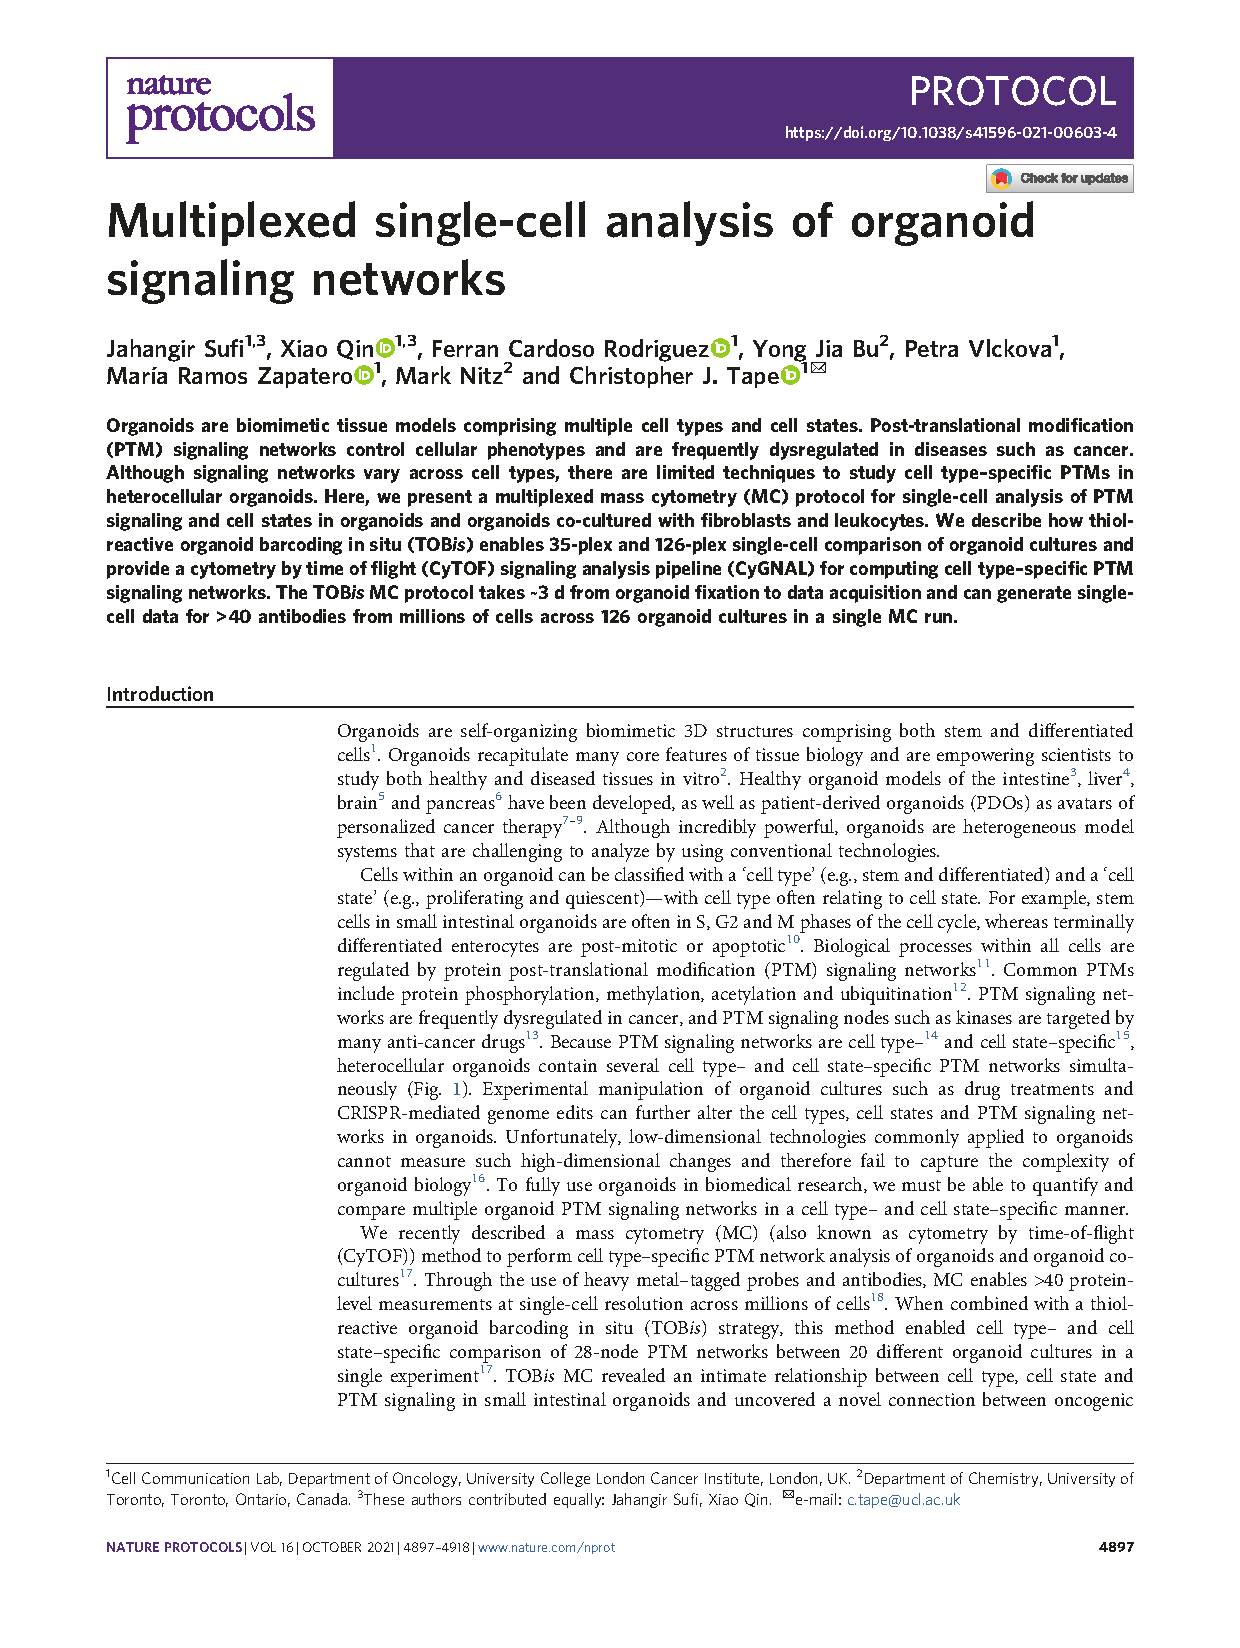
\includepdf[pages={1-22}, scale=1, offset=24mm -28mm]{0Xappendices/sufiqin.pdf}


\chapter{Colophon}
\label{appendix:colophon}

This Thesis has been written with \LaTeX and its figures assembled using the FOSS vector graphics editor Inkscape (\url{inkscape.org}). Resources used for making figures include plots generated from code (R and Python), \emph{de novo} drawn graphics, and graphics altered from the open source Bioicons resource (\url{bioicons.com}). 

The Thesis is currently hosted in GitHub as a private repository. However, once the sections of work currently under revision at Cell are part of the public domain, I will make the repository public. Code availability covers all chapters and is distributed along multiple GitHub repositories.
